% !TEX root = MAIN.tex

\section{Introduction}
\label{sec:introduction}
\addcontentsline{toc}{chapter}{Introduction}

%This document is the summary report of the ESA activity ITT-1-9873-ESA, which concerns the development of a framework for the automated assessment and the automated improvement of test suites for space software\footnote{In this report, we use the term space software to indicate software to be deployed on hardware that runs on-orbit.}.
 
From spacecrafts to ground stations, software has a prominent role in space systems; for this reason, the success of space missions depends on the quality of the system hardware as much on the dependability of its software. Mission failures due to insufficient software sanity checks~\cite{Schiaparelli} are unfortunate examples, pointing to the necessity for systematic and predictable quality assurance procedures in space software. 


Since one of the primary objectives of software testing is to identify the presence of software faults, an effective way to assess the quality of a test suite consists of artificially injecting faults in the software under test and verifying the extent to which the test suite can detect them. 
This approach is known as \emph{mutation analysis}~\cite{DeMillo78}. 
In mutation analysis, faults are automatically injected in the program through automated procedures referred to as mutation operators. Mutation operators enable the generation of faulty software versions that are referred to as \emph{mutants}.  
Mutation analysis helps evaluate the effectiveness of a test suite, \JMRCHANGE{for a specific software system,} based on its mutation score, which is the percentage of mutants leading to test failures. Also, mutation analysis enables \emph{mutation testing}, which concerns the automated generation of test cases that discover mutants.

Despite its potential, mutation analysis is not widely adopted by industry. The main reasons include its limited scalability and the pertinence of the mutation score as an adequacy criterion~\cite{papadakis2016threats}. Indeed, for a large software system, the number of generated mutants might prevent the execution of the test suite against all the mutated versions. Also, the generated mutants might be either 
semantically equivalent to the original software~\cite{madeyski2013overcoming} or redundant with each other~\cite{Shin:TSE:DCriterion:2018}. Equivalent and redundant mutants may bias the mutation score as an adequacy criterion. 
Finally, test generation approaches are preliminary and cannot be applied in industrial space context. For example, they can generate test inputs only for batch programs that can be compiled with the LLVM infrastructure~\cite{chekam2021killing}.

%The mutation analysis literature has proposed several optimizations to address problems related to scalability and mutation score pertinence~\cite{zhang2013operator,gopinath2015hard,zhang2013faster,grun2009impact,schuler2010covering,schuler2013covering,schuler2009efficient}. 
%However, these approaches 
%have not been evaluated on industrial, embedded systems
%and there are no feasibility studies concerning the integration of such optimizations and their resulting, combined benefits.
%Also, existing mutation analysis approaches cannot identify problems related to the interoperability of integrated components (integration testing), which is a major problem in 
%Cyber-physical Systems~\cite{Givehchi:2017,Jirkovsk:2017} and, consequently, space software --- mainly due to the wide variety and heterogeneity of the technologies and standards adopted.

The FAQAS activity addresses the problems above. It is a joint work between the SnT Centre of the University of Luxembourg\footnote{https://wwwen.uni.lu/snt}, Gomspace Luxembourg\footnote{https://gomspace.com/} (GSL) and OHB Luxspace\footnote{https://luxspace.lu/} (LXS).
FAQAS led to the development of a toolset that addresses the challenges above. It includes four tools:
\EMPH{MASS} (Mutation Analysis for Space Software), 
\EMPH{DAMAt} (DAta-driven Mutation Analysis with Tables), 
\EMPH{SEMuS} (Symbolic Execution-based MUtant analysis for Space software),
and \EMPH{DAMTE} (DAta-driven Mutation TEsting).



% of code-driven mutation analysis in the space context. The evaluation has shown that the most effective solutions to improve scalability and mutation score accuracy are mutants sampling and equivalence metrics based on compiler optimizations, respectively. To guarantee a scalable mutation testing process and the accurate computation of the mutation score, mutants sampling should be based on sequential analysis relying on fixed-width sequential confidence interval, a research discovery done within FAQAS.
%
%•	An empirical evaluation demonstrating the feasibility of data-driven mutation analysis with space software.
%•	The definition of an approach for code-driven mutation testing that relies on symbolic execution to identify test inputs that enable killing mutants not killed by the test suite under analysis.
%•	Demonstrating the feasibility of automated test generation for mutation testing based on symbolic execution. More precisely, symbolic execution can be successfully used to select test inputs that kill live mutants within unit test cases. However, unsurprisingly, it cannot be adopted when, to kill a mutant, it is necessary to rely on external components (e.g., networks or simulators), in such cases, which are common for integration and system test suites, symbolic execution alone is insufficient to generate test cases (e.g., because it cannot translate the simulator logic into an SMT formula to derive test cases from).
%\item The definition of guidelines for the adoption of mutation analysis and testing strategies within ECSS activities. The proposed guidelines support both quality assurance activities described in ECSS standards and Independent Software Verification and Validation (ISVV) practices.
%\end{itemize}

\begin{figure*}[tb]
\begin{center}
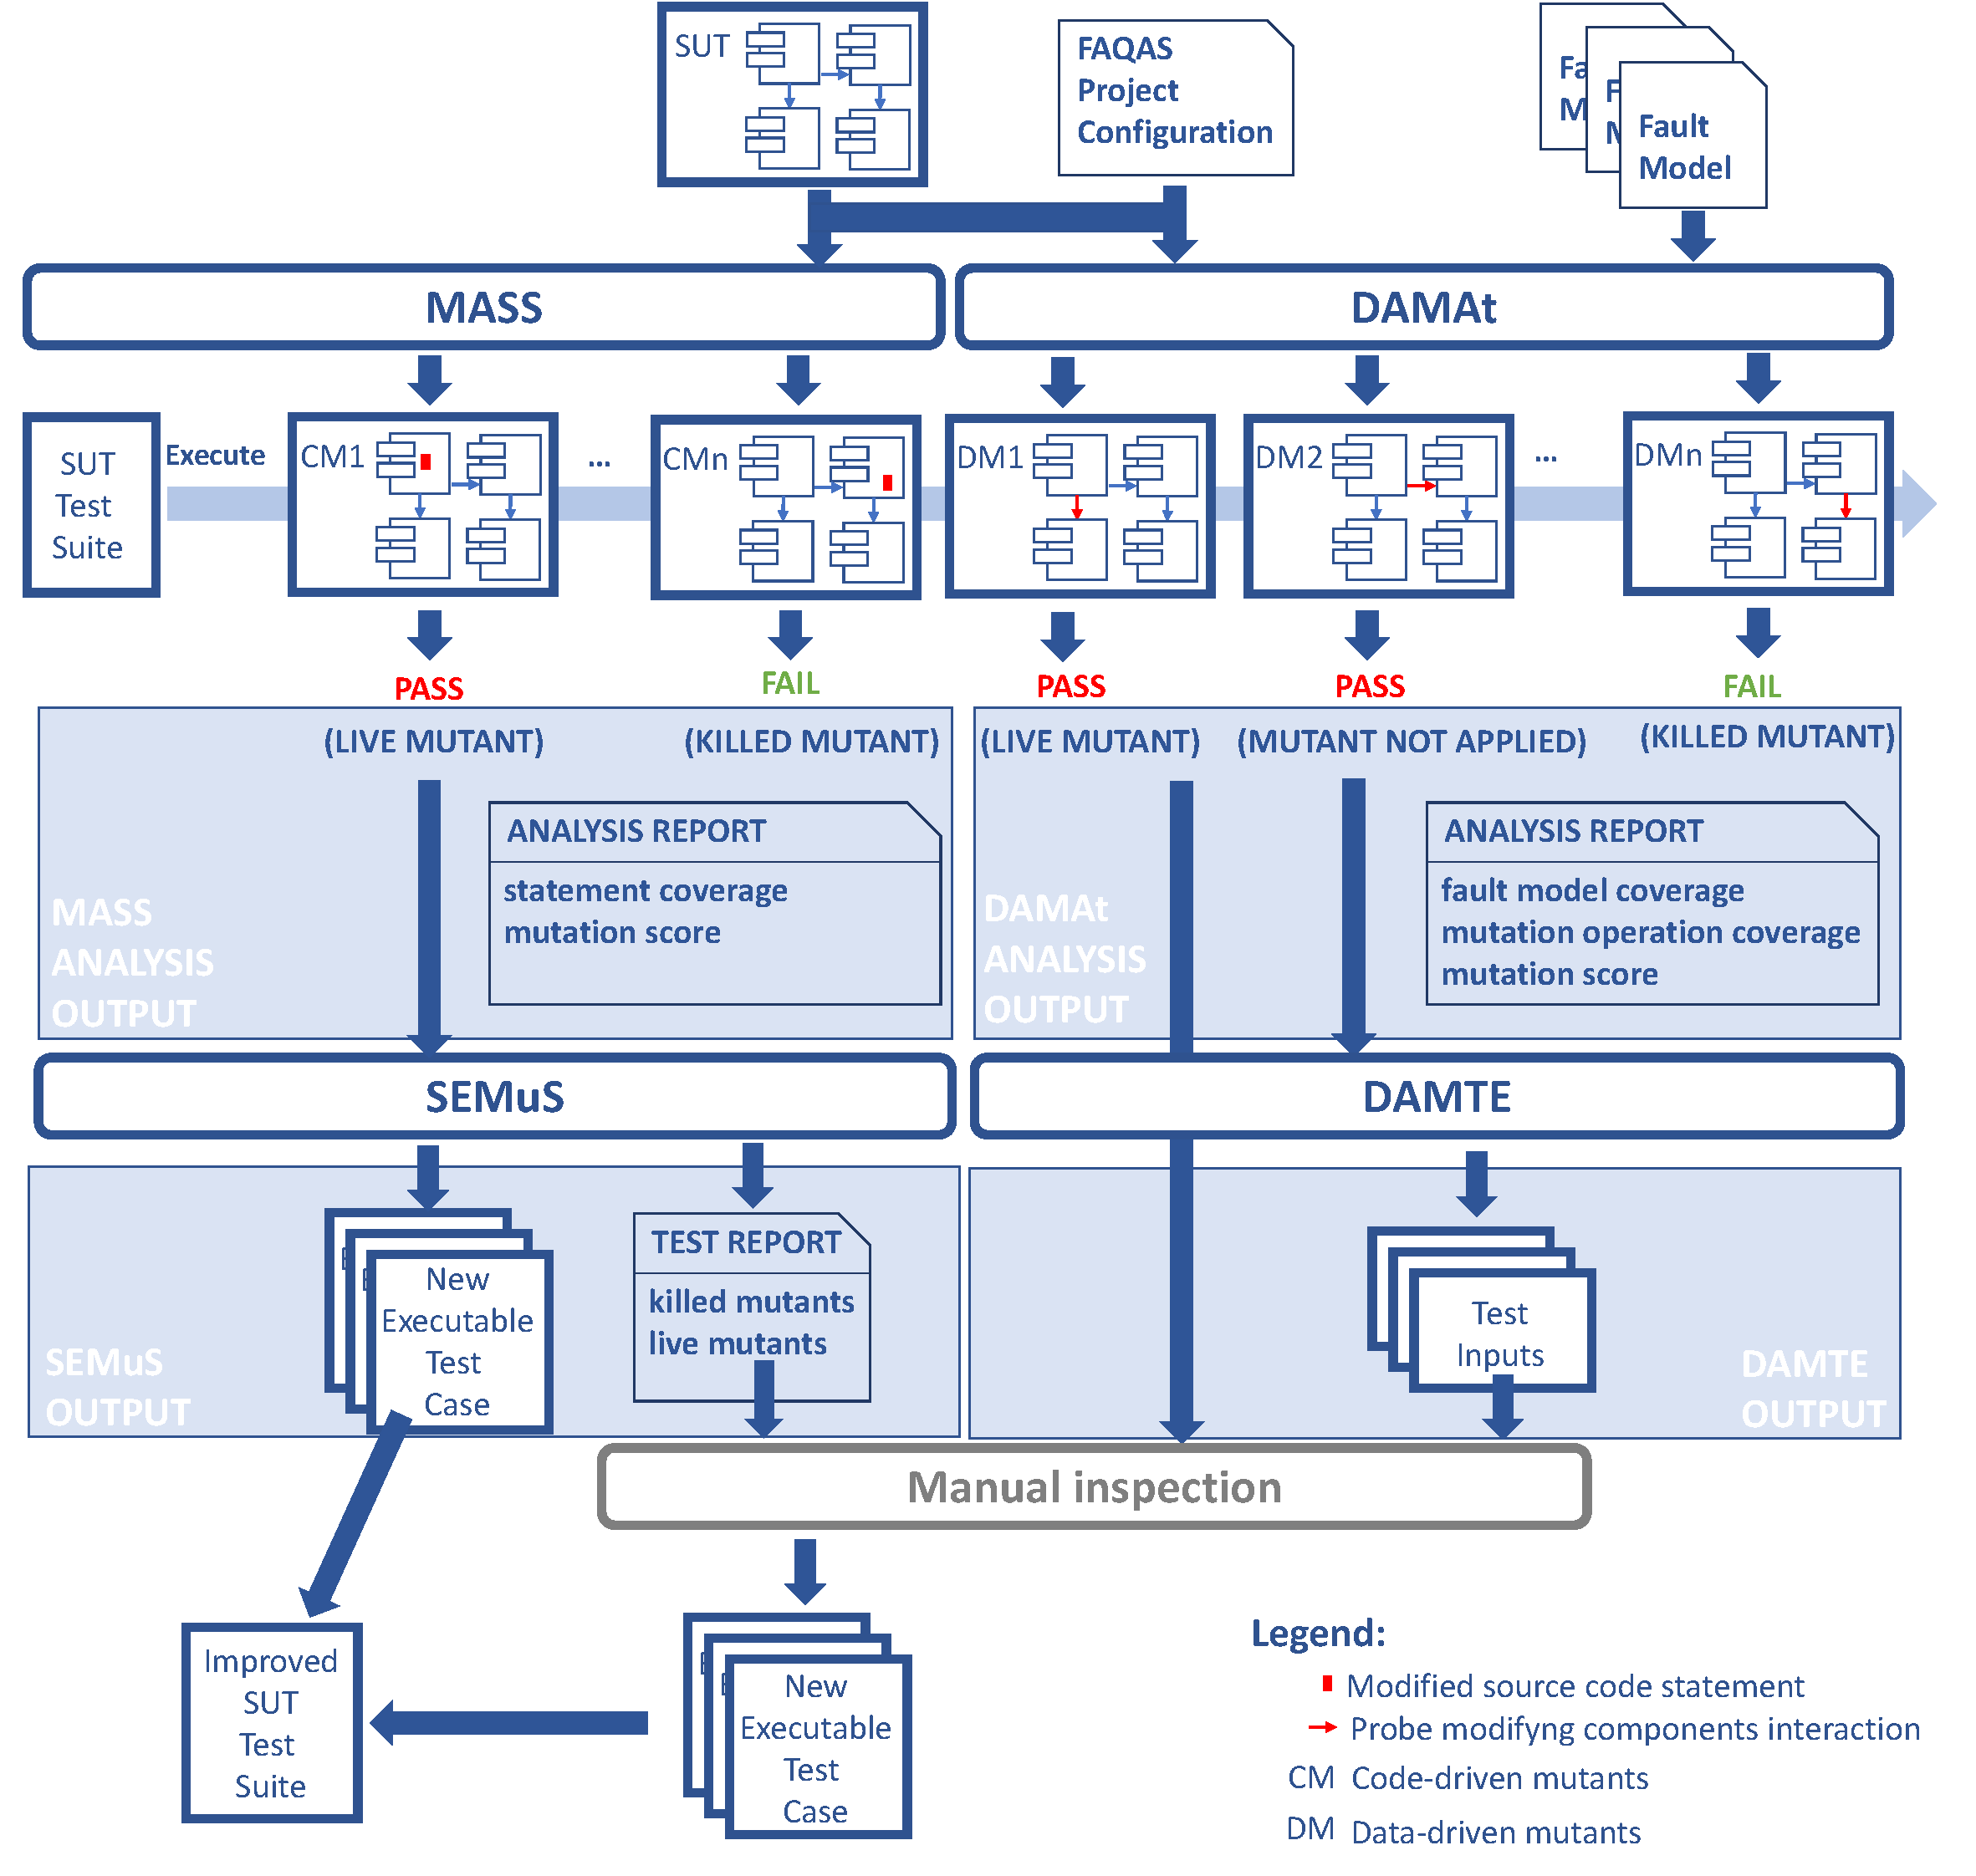
\includegraphics[width=0.7\textwidth]{images/FAQAS-overview.pdf}
\caption{Overview of the FAQAS toolset}
\label{fig:FAQAS:toolset}
\end{center}
\end{figure*}

Figure~\ref{fig:FAQAS:toolset} provides an overview of the input and outputs of the FAQAS toolset. It relies on the idea of generating multiple modified versions of the software system under test (SUT), some are derived by modifying the implementation of the software (code-driven mutants) other by integrating a mutation API that alters the messages exchanged by the software components of the SUT (data-driven mutants). 
The SUT test suite shall be executed with all the mutants, if it is effective then it shall fail with each of them. The mutants for which a failure is not observed are said to be \EMPH{live} and indicate a pitfall in the test suite.
All the FAQAS tools take as input the software under test (SUT), its test suite, and a set of configuration files. 

\EMPH{MASS} generates code-driven mutants. It integrates a pipeline of solutions that make mutation analysis feasible with large SUT. The three main contributions of MASS are (1) the automated identification of trivially equivalent mutants using an ensemble of compiler optimization options, (2) the computation of the mutation score based on mutant sampling with fixed size confidence interval approach (FSCI), (3) the automated identification of equivalent mutants based on coverage. 
MASS reports the set of live mutants, the set of killed mutants (i.e., mutants that are discovered by the test suite), and information useful to draft a verification report, which includes the statement coverage of the SUT test suite and the mutation score (i.e., the percentage of mutants discovered by the test suite).

\EMPH{DAMAt} generates mutants for data-driven mutation analysis. Data-driven mutation analysis is a research contribution of FAQAS. Instead of mutating the implementation of the SUT, it consists of altering the data exchanged by software components. 
DAMAt relies on fault models that specify how to mutate the data exchanged by software components through data-driven mutation operators. DAMAt can automatically alter data that is stored in data buffers (e.g., before serialization on the communication channel).
DAMAt enables the simulation of faults that affect simulated components (e.g., sensors), which is not feasible with traditional, code-driven mutation analysis. 
DAMAt generates as output a set of killed mutants (i.e., mutants that, during testing, successfully alter the data, and lead to test case failures), a set of live mutants (i.e., mutants that, during testing, successfully alter the data, but do not lead to test case failures), and a set of mutants not applied (i.e., mutants that, during testing, could not alter any data because the data they target is never exercised by the SUT); also, it provides information useful to draft a verification report, which includes the fault model coverage (i.e., percentage of fault models with at least one mutant applied), the mutation operation coverage (i.e., percentage of mutants applied), and the mutation score.

\EMPH{SEMuS} automatically generates executable unit test cases based on code-driven mutation analysis results. The generated unit test cases detect mutants not detected by the original test suite. The generated test cases include test oracles that shall be manually validated by engineers, which enables detecting faults. The generated test cases can be integrated into regression test suites.

SEMuS takes as input the list of live mutants detected by MASS. It generates a set of additional test cases that can be integrated into the SUT test suite. Also, it reports the list of killed mutants and the list of mutants that remain live (i.e., for which SEMuS did not generate a test case that kill them). Live mutants shall be manually inspected by engineers to either determine if they are equivalent or to manually derive a test case capable of killing them.

\EMPH{DAMTE} is a manual procedure supported by an automated symbolic execution toolset; it automatically identifies the test inputs that make software components exchange the data targeted by data-driven mutation operators. The derived test inputs can then be manually integrated into the SUT test suite.
 
The activity also included an extensive empirical evaluation demonstrating the feasibility, effectiveness, and scalability of the proposed toolsets in the space context, as described in the following sections.
 
%FAQAS.drawio.pdf

%Sections~\ref{ch:mass:approach} to~\ref{sec:data:test_suite_augmentation} provide an overview of the FAQAS tools: MASS, SEMuS, DAMAt, and DAMTE.
%Section~\ref{chapter:caseStudies} introduces the case study subjects considered for empirical evaluation.
%Section~\ref{sec:summary:results} provides an overview of the empirical results obtained.
%Section~\ref{sec:conclusion} concludes this report.

